\subheading{Wherein the Model and Measured Are Compared}
\section*{Section Five (a)}

Another test of the model was to compare it to the measured Bode plot.  Getting
the model values was easily accomplished by taking the transfer function from
Equation \eqref{transfer-function} and substituting the known $C$ and $\beta$
values into it.  Getting the measured values was a little more difficult, in the
end the method chosen was the same as that used to getting the model values; at
each frequency the identification function was used to get the average $C$ and
$\beta$ values from that data set, then the transfer function derived from the
value was evaluated at that frequency.

Figure \ref{5a} shows the magnitude and phase plots found, along with the
absolute relative error.  As can be seen these plots are quite accurate, there
is less than 17\% error in the magnitude and less than ??\% error in phase.

\includefigure{width=0.8\textwidth}
              {images/section-5a}
              {Bode plot and error plot of the model vs measured\label{5a}}

\subheading{Wherein All the Models Are Compared}
\section*{Section Five (b)}

To ensure that the model chosen was the best of the available models the rest of
the data sets were also used to derive a model, then the Bode plots of these
were all compared to the measured data.  The results of the comparison can be
seen in Figure \ref{5b-1}.  This shows that all the models have very good
magnitude responses at low frequencies, but as they approach the bend they
diverge quite a bit from the measured values before settling into a path pretty
much parallel to the correct values.  They are all quite a bit better in the
phase response, but none of them really manage to distinguish themselves by
being amazingly better.

To help parse the info contained in the comparison an additional plot show in
Figure \ref{5b-2} was created.  This shows the sum of the errors from the last
figure at each frequency for both magnitude and phase.  From this it can be seen
that there are two models with much better magnitude response than the rest,
these are models 7 and 8 at frequencies of 1.8 and 2.0 Hz.  Out of these 7 has a
better phase response, so we can now see why it was chosen as the model to use
from the start.

Figure \ref{5b-3} also shows the $C$ and $\beta$ values found for each model.

\includefigure{width=0.8\textwidth}
              {images/section-5b-1}
              {Bode plot and error plot of all models\label{5b-1}}

\begin{figure}
  \begin{minipage}{0.5\linewidth}
    \centering
    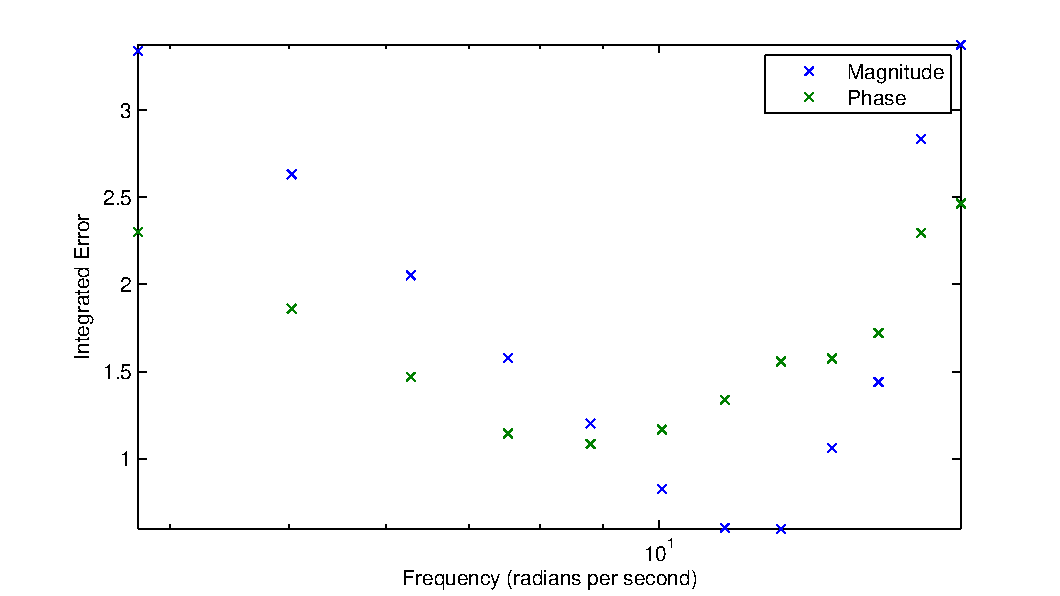
\includegraphics[width=\textwidth]{images/section-5b-2}
    \caption{\small Integrated errors of each model\label{5b-2}}
  \end{minipage}
  \begin{minipage}{0.5\linewidth}
    \centering
    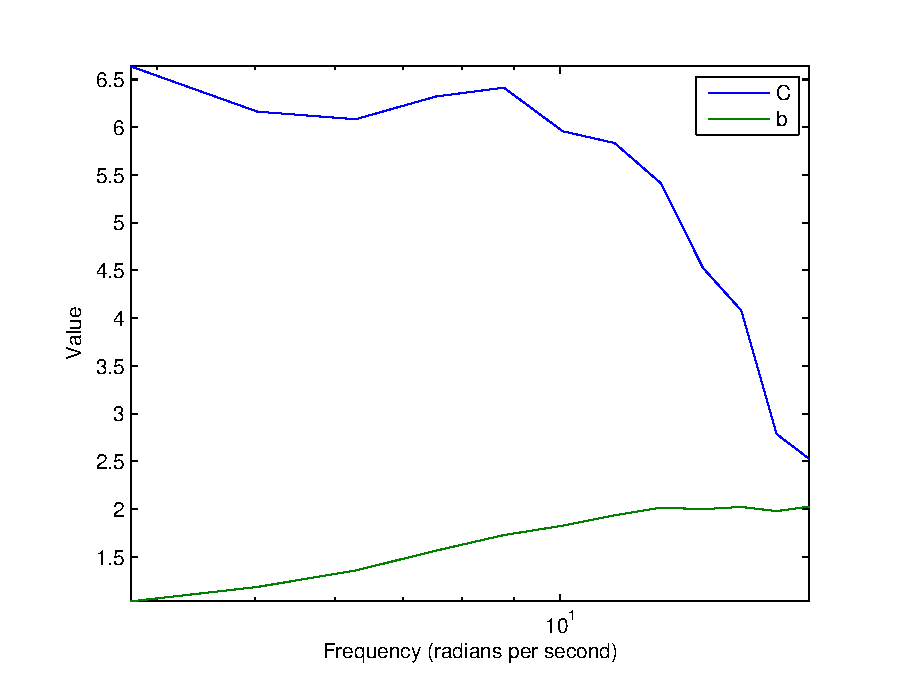
\includegraphics[width=\textwidth]{images/section-5b-3}
    \caption{\small$C$ and $\beta$ values of each model\label{5b-3}}
  \end{minipage}
\end{figure}
